\chapter{Simulations and Results}
For all simulations, a 1000x1000 square is used to represent the whole 2-D plane. This size is good enough in the sense that using a larger square led to longer runtimes with little to no 
effect on the results. In the mobility model we used, transition length is Rayleigh distributed. To draw a length from Rayleigh distribution, the following method is used:

\begin{enumerate}
	\item Draw a number N from Poisson distribution with density $\lambda A$ where $A$ is the area of the square.
	\item Spread these N points uniformly on the plane
	\item Of these N points, choose the point that is closest to the point under consideration. 
\end{enumerate}

As discussed in \cite{ganti}, this leads to Rayleigh distribution of transition length and can be proved easily using null probability of a Poisson Point Process. 
\begin{figure}[h]
	\centering \vspace{-0.1in}
	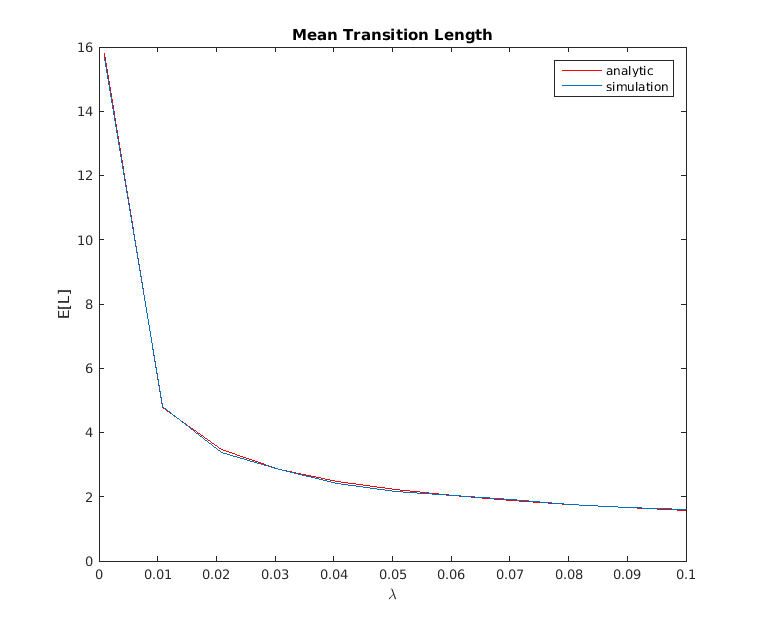
\includegraphics[width=0.75\textwidth]{images/rwpStat.png}
	\vspace{-20pt} \caption[Effect of the proximal Operator]{\small Effect of the Proximal Operator }
	\label{fig:rwpEL}
\end{figure}

\begin{comment}
\begin{figure}[h]
	\centering \vspace{-0.1in}
	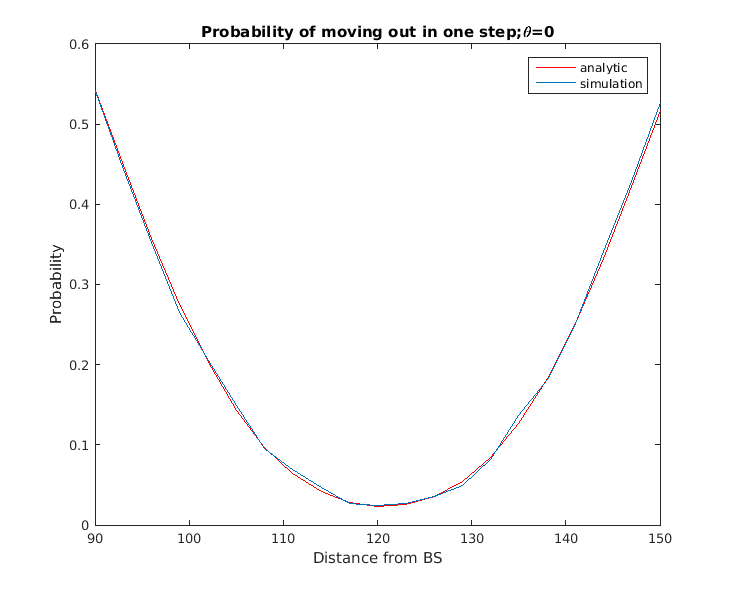
\includegraphics[width=0.75\textwidth]{images/oneOutProb0.png}
	\vspace{-20pt} \caption[Effect of the proximal Operator]{\small Effect of the Proximal Operator }
	\label{fig:oneOut0}
\end{figure}

\begin{figure}[h]
	\centering \vspace{-0.1in}
	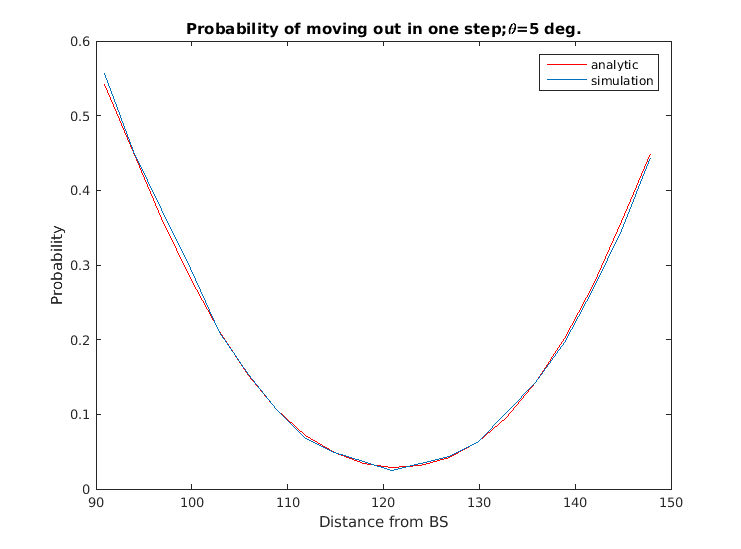
\includegraphics[width=0.75\textwidth]{images/oneOutProb5.png}
	\vspace{-20pt} \caption[Effect of the proximal Operator]{\small Effect of the Proximal Operator }
	\label{fig:oneOut5}
\end{figure}

\begin{figure}[h]
	\centering \vspace{-0.1in}
	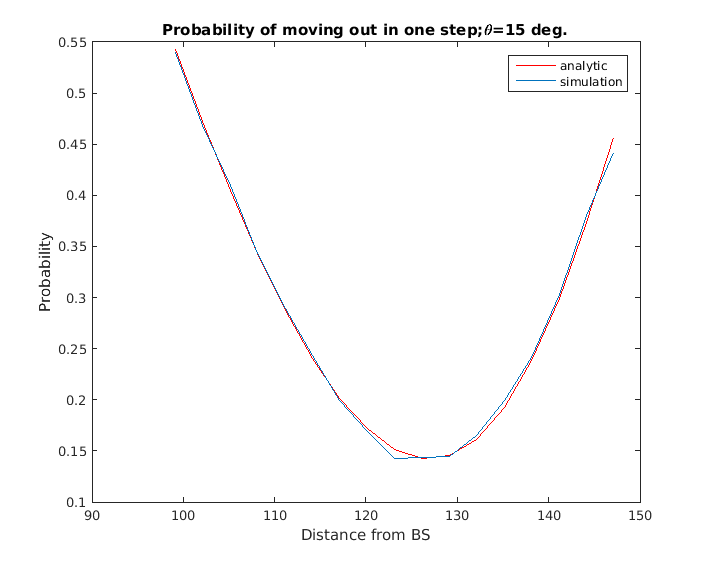
\includegraphics[width=0.75\textwidth]{images/oneOutProb15.png}
	\vspace{-20pt} \caption[Effect of the proximal Operator]{\small Effect of the Proximal Operator }
	\label{fig:oneOut15}
\end{figure}

\begin{figure}[h]
	\centering \vspace{-0.1in}
	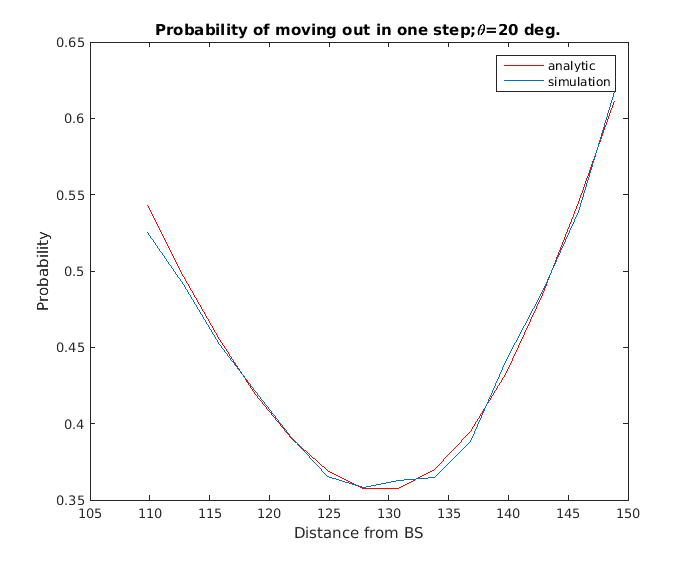
\includegraphics[width=0.75\textwidth]{images/oneOutProb20.png}
	\vspace{-20pt} \caption[Effect of the proximal Operator]{\small Effect of the Proximal Operator }
	\label{fig:oneOut20}
\end{figure}
\end{comment}


\begin{figure}[ht!]
     \begin{center}
%
        \subfigure[Caption of First Figure]{%
            \label{fig:first}
            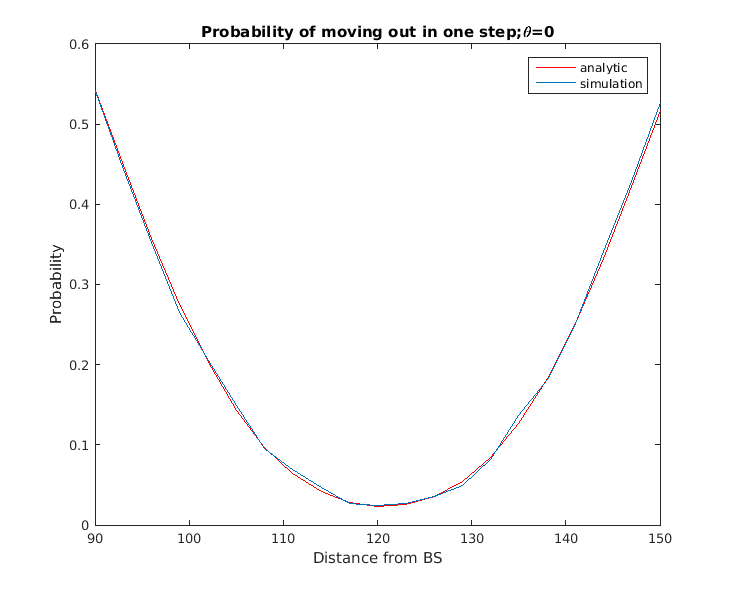
\includegraphics[height = 2.5in,width=3.5in]{images/oneOutProb0.png}
        }%
        \subfigure[Caption of Second Figure]{%
           \label{fig:second}
           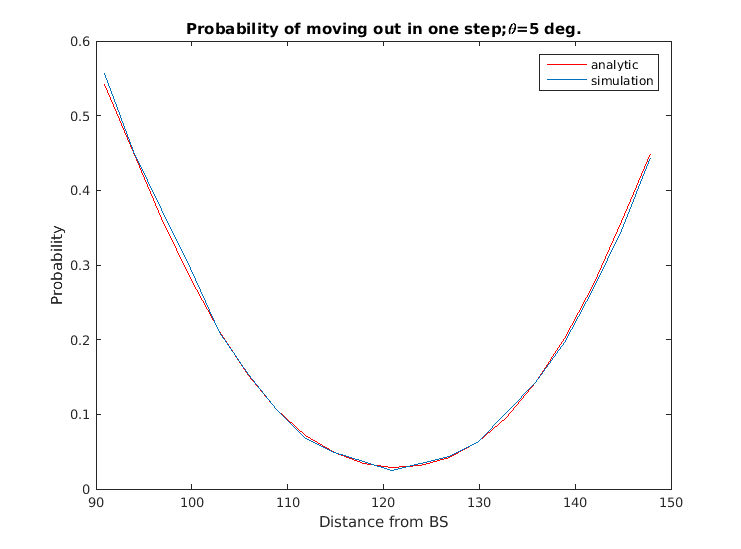
\includegraphics[height = 2.5in,width=3.5in]{images/oneOutProb5.png}
        }\\ %  ------- End of the first row ----------------------%
        \subfigure[Caption of Third Figure]{%
            \label{fig:third}
            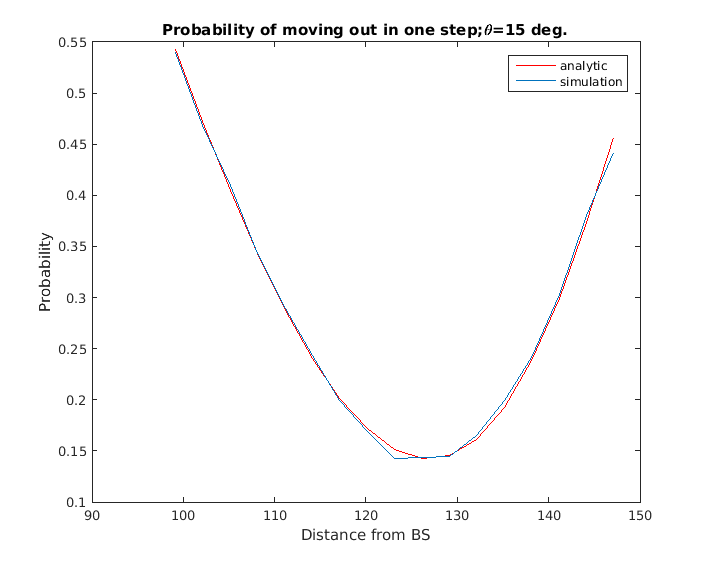
\includegraphics[height = 2.5in,width=3.5in]{images/oneOutProb15.png}
        }%

        \subfigure[Caption of Fourth Figure]{%
            \label{fig:fourth}
            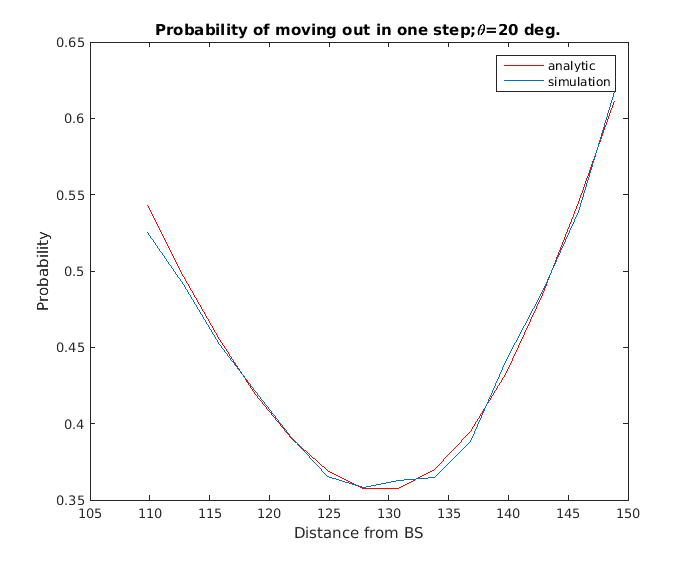
\includegraphics[height = 2.5in,width=3.5in]{images/oneOutProb20.png}
        }%
%
    \end{center}
    \caption{%
        The l-o-n-g caption for all the subfigures
        (FirstFigure through FourthFigure) goes here.
     }%
   \label{fig:subfigures}
\end{figure}

\begin{figure}[ht!]
     \begin{center}
%
        \subfigure[Caption of First Figure]{%
            \label{fig:first}
            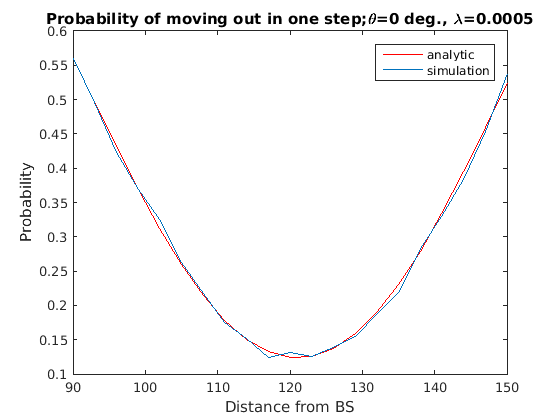
\includegraphics[width=0.6\textwidth]{images/oneOutProbl0005t0.png}
        }%
        \subfigure[Caption of Second Figure]{%
           \label{fig:second}
           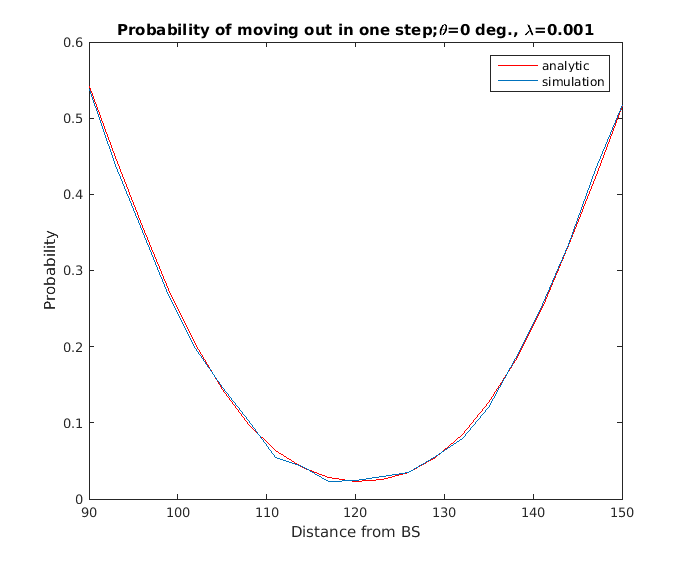
\includegraphics[width=0.55\textwidth]{images/oneOutProbl001t0.png}
        }\\ %  ------- End of the first row ----------------------%
        \subfigure[Caption of Third Figure]{%
            \label{fig:third}
            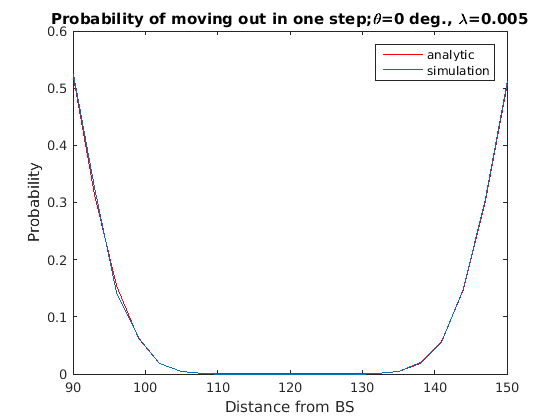
\includegraphics[width=0.6\textwidth]{images/oneOutProbl005t0.png}
        }%

%        \subfigure[Caption of Fourth Figure]{%
%            \label{fig:fourth}
%            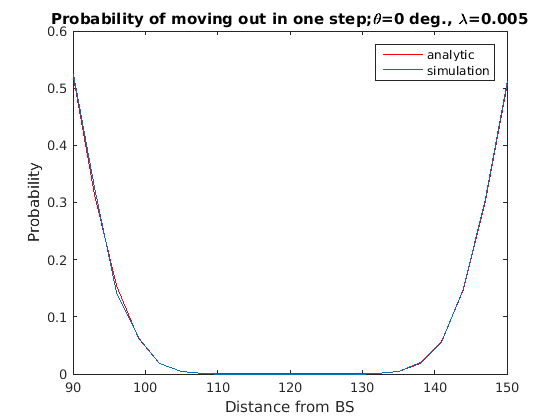
\includegraphics[width=0.4\textwidth]{images/oneOutProbl005t0.png}
        %}%
%
    \end{center}
    \caption{%
        The l-o-n-g caption for all the subfigures
        (FirstFigure through FourthFigure) goes here.
     }%
   \label{fig:subfigures}
\end{figure}
